\documentclass{article}
\usepackage{../fasy-hw}
\usepackage{ wasysym }

%% UPDATE these variables:
\renewcommand{\hwnum}{6}
\title{Advanced Algorithms, Homework \hwnum}
\author{Nathan Stouffer}
\collab{n/a}
\date{due: 26 October 2020}

\begin{document}

\maketitle

In any question that you are expected to provide an algorithm, you are
expected to provide:
\begin{enumerate}
    \item Describe the problem in your own words, including describing what the input and output is.
    \item Describe, in paragraph form, the algorithm you propose.
    \item Provide a nicely formatted algorithm to solve the problem.
    \item Use a decrementing function to prove that algorithm terminates OR  Give the runtime with justification.
    \item Prove partial correctness.
    In other words, if there is a loop or recursion, what is the loop/recursion invariant? Provide the proof.
    (Note: you only need to do this for the outer-most loop if there are nested loops).
\end{enumerate}



\nextprob
\collab{n/a}

Walk through Kruskal's algorithm, using the graph in Figure 7.7 (left) of the
textbook.  Label the center vertex $a$, the other red vertex $b$, and the
remainder $c$ through $g$ in counter-clockwise order.  You should use the
union-find data structure, with both ``heuristics.''

\paragraph{Answer}

% ============================================

Here is my walk through:

\begin{figure}[h]
    \begin{center}
        \includegraphics[scale=0.1]{img/kruskal-walk-through}
        \caption{Walking through Kruskal's algorithm}
        \label{fig:kruskal}
    \end{center}
\end{figure}

% ============================================

\nextprob
\collab{n/a}

Chapter 3, Question 9 (Palindromes)

A palindrome is any string that is exactly the same as its reversal.

Any string can be decomposed into a sequence of palindromes.
Describe and analyze an efficient algorithm to find the smallest number of palindromes that make up a given input string.

\paragraph{Answer}

% ============================================

\begin{enumerate}
    \item The input to this problem is an array containing a string of characters.
    The goal is to find the smallest number of palindromes that concatenate to form the input string.
    For output, we will give an integer (the smallest integer number of palindromes that make the input string).
    \item My algorithm works in two parts.
    First I will describe the recursive portion of the algorithm, and then (to make it efficient) I will discuss how to reach the dynamic programming solution.
    The recursive algorithm starts at the beginning of the string.
    If we have a pointer to a letter in the string, that letter must be part of a palindrome which precedes it or it must start a new palindrome.
    Then we recursively compute the number of palindromes in each case to find the total number of palindromes that compose the input.
    Then we take the minimum value. \parspace
    The algorithm I just described runs in expnonential time since it either chooses to include a letter or not include it.
    However we would like this algorithm to be efficient.
    To do so, we employ dynamic programming.
    If the pointer to the current string is at index $f$ and the beginning of the palindrome containing word[$f$] is at index $s$.
    Then we can say that the decision for $s,f$ depends on the decision for $s,f+1$ and $f+1,f+1$.
    This induces a dynamic programming algorithm that runs in polynomial time (the size of the table), so we have an efficient algorithm!
    \item Here is the psuedocode of the recursive algorithm.
    \begin{algorithm}
        \textsc{PalinSeq}(word, s, f) \\
        1. \hspace{1em} if (f $>$ len(word)) \\
        2. \hspace{2em}     if (\textsc{IsPalin}(word, s, f-1)) \\
        3. \hspace{3em}         return 1 \\
        4. \hspace{2em}     else \\
        5. \hspace{3em}         return $+\infty$ \\
        6. \hspace{1em} cur = \textsc{PalinSeq}(word, s, f+1) \\
        7. \hspace{1em} nxt = $+\infty$ \\
        8. \hspace{1em} if (\textsc{IsPalin}(word, s, f)) \\
        9. \hspace{2em}     nxt = 1 + \textsc{PalinSeq}(word, f+1, f+1) \\
        10. \hspace{0.75em} return min (cur, next)
    \end{algorithm} \\
    From here, we can use the following dynamic programming table to build our efficient solution (arrows drawn because of the dependency on $T[s,f+1]$ and $T[f+1,f+1]$):
    \begin{figure}
        \begin{center}
            \includegraphics[scale=0.1]{img/dp-table}
            \caption{Dependency Table for $n=4$}
		    \label{fig:dynprog}
        \end{center}
    \end{figure}
    \newpage
    \item We will use a decrementing function to show that the recursive version terminates.
    This implies termination for the dynamic programming solution.
    Let our state space be letters in the variable word.
    Our map to the natural numbers is the number of letters following the index f+1.
    The function is strictly decreasing because becuase each iteration sends in $f_1 + 1$ for $f_{i+1}$.
    This implies termination because our stopping condition is that $f > len(word)$.
    \item Now suppose that our algorithm terminates, why should it be correct?
    Again, we need only show correctness of the recursive solution for the dynamic program to also be correct.
    The recursive solution is correct because we test every possibility for sequences of palindromes and take the minimum value.
    Then the dynamic program evaluates the program in an intelligent way instead of testing all possibilities.
\end{enumerate}

% ============================================

\nextprob
\collab{n/a}

Chapter 7, Question 1 (Shortest and Longest Edges in Cycle)

Let $G = (V, E)$ be an arbitrary connected graph with weighted edges.
\begin{enumerate}[label=(\alph*)]
    \item Prove that for any cycle in $G$, the minimum spanning tree of $G$ excludes the maximum-weight edge in that cycle.
    \item Prove or disprove: The minimum spanning tree of $G$ includes the minimum-weight edge in every cycle in $G$.
\end{enumerate}

\paragraph{Answer}

% ============================================

\begin{enumerate}[label=(\alph*)]
    \item We will prove that given a cycle in $G$, the minimum spanning tree of $G$ does not include the maximum-weight edge in that cycle.
    To this end, pick a cycle $C$ and label the maximum-weight edge $e_{max}$.
    Now suppose we have some spanning tree $T$ that includes $e_{max}$.
    Now we show that $T$ is not the minimum spanning tree for $G$. \parspace
    Since $C$ is a cycle, there exists some edge $e \in C$ that is not contained in $T$ (otherwise $T$ would not be a tree) and that connects the same components that $e_{max}$ connects.
    We know that $e \neq e_{max}$ since $e$ is not contained in $T$.
    Then, by definition of $e_{max}$, we must have $weight(e) < weight(e_{max})$.
    Now let $T' = T - e_{max} + e$.
    Certainly the total weight of $T'$ is less than the total weight of $T$.
    If $T'$ is a spanning tree, then $T$ is certainly not the minimum spanning tree.
    $T'$ must be a spanning tree because $e$ connects the same components that $e_{max}$ connects.
    Therefore, $T$ cannot be a minimum spanning tree since another spanning tree of $G$ exists with less weight.
    \item The minimum spanning tree of $G$ does not necessarily have to include the minimum-weight ege in every cycle of $G$.
    Consider the following counterexample:
    \begin{center}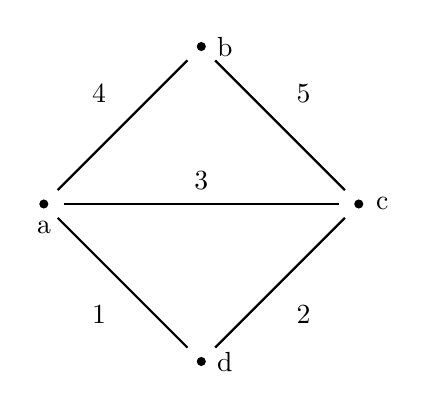
\begin{tikzpicture}[scale=2]
    %% vertices
    \draw [fill=black] (0.0,0.0)     circle (0.025);
    \draw [fill=black] (1.0,1.0)     circle (0.025);
    \draw [fill=black] (2.0,0.0)     circle (0.025);
    \draw [fill=black] (1.0,-1.0)    circle (0.025);
    %% labels
    \node at (0.0,-0.15) {a};
    \node at (1.15,1.0) {b};
    \node at (2.15,0.0) {c};
    \node at (1.15,-1.0) {d};
    %% weights
    \node at (0.35,-0.7) {1};
    \node at (1.65,-0.7) {2};
    \node at (1,0.15) {3};
    \node at (0.35,0.7) {4};
    \node at (1.65,0.7) {5};

    %% edges
    \draw [thick] (0.088,0.088) -- (0.912,0.912);
    \draw [thick] (0.125,0.0) -- (1.875,0.0);
    \draw [thick] (0.088,-0.088) -- (0.912,-0.912);
    \draw [thick] (1.088,0.912) -- (1.912,0.088);
    \draw [thick] (1.912,-0.088) -- (1.088,-0.912);
\end{tikzpicture}
\end{center}
    Consider the cycle $a \to b \to c \to a$ which has minimum-weight edge $ac$.
    But the above graph has minimum spanning tree with edges $ad, dc, ab$.
    The minimum spanning tree does not contain $ac$ so we have found a counterexample.
\end{enumerate}

% ============================================


\nextprob
\collab{n/a}

Chapter 8, Question 3 (Weights on Vertices)

Suppose we are given an undirected graph $G$ in which every vertex has a positive weight.
\begin{enumerate}[label=(\alph*)]
    \item Describe and analyze an algorithm to find a spanning tree of $G$ with minimum total weight.
    \item Describe and analyze an algorithm to find a path in $G$ from one given vertex $s$ to another given vertex $t$ with minimum total weight.
\end{enumerate}

\paragraph{Answer}

% ============================================
\begin{enumerate}[label=(\alph*)]
    \item We first describe and analyze an algorithm to find a spanning tree of $G$ with minimum total weight.
        \begin{enumerate}[label=\alph*)]
            \item The input to the problem is a connected, undirected graph $G = (V, E)$ paired with a weight function $w: V \rightarrow \R ^+$.
            We define the weight of a graph $G$ to be $weight(G) = \sum _{v \in V} w(v)$. \parspace
            The output will be a tree with minimum weight $T = (V_T, E_T) \subset G$ such that every vertex of $V$ is in $T$ and $T$ is connected.
            In this problem, every vertex must be contained in $T$ so the weight of every spanning tree is the same value.
            \item Since every spanning tree of $G$ will have the same weight, we need only provide an algorithm that computes a spanning tree $T$ of $G$.
            To do this, we will use a union-find data structure.
            First, we will initialize the data structure with every vertex in its own component.
            Then we will iterate over every edge.
            For each edge $e = (s, t)$, we will test if $s$ and $t$ are in the same component.
            If not, union them in the data structure and add $e$ to $T$.
            After iterating through the edges, $T$ will be a miminum spanning tree for $G$.
            \item Here is the algorithm:
            \begin{algorithm}
                \textsc{MST}($G = (V, E)$) \\
                1. \hspace{1em} $T = (V, \emptyset)$ \\
                2. \hspace{1em} uf = init($V$) \\
                3. \hspace{1em} for $i=1..|E|$ \\
                4. \hspace{2em}     $(s_i, t_i) = E[i]$ \\
                5. \hspace{2em}     if (uf.find($s_i$) $\neq$ uf.find($t_i$)) \\
                6. \hspace{3em}         uf.union($s_i, t_i$) \\
                7. \hspace{3em}         $T = T \cup (\emptyset, (s_i, t_i)) $       // add edge to tree \\
                8. \hspace{1em} return $T$
            \end{algorithm}
            \item We prove that \textsc{MST} terminates by giving a run time analysis.
            Line 1 takes constant time and line 2 takes $\Theta (V)$ time.
            Line 3 runs exactly $|E|$ times and lines 4, 7, and 8 all run in constant time.
            This leaves only lines 5 and 6 unaccounted for.
            If we use the heuristic version of union find, then both lines run in constant time.
            Therefore the run time of the algorithm is a composition of polynomials, which is finite and the algorithm must terminate.
            \item We now prove partial correctness.
            Suppose that \textsc{MST} terminates, will it terminate in a correct state?
            We will define a loop invariant for the loop beginning on line 3.
            At iteration $i$, the loop invariant $L_i$ is that $T_i$ is a forest of the connected components of $G$ after processing the first $i$ edges.
            Prior to the for loop, we have not processed any edges so $T$ should just contain every vertex in its own connected component, which is the case.
            As we are processing the for loop, an edge is added to $T$ only if the vertices are found to be in different components, thus connecting the components and preserving the forest structure of $T$.
            After the for loop terminates (which we know will occur because we proved termination), we will have processed every edge.
            Then $T$ is not a forest, but a single tree since the graph $G$ is assumed to be connected.
            Additionally, $T$ is a spanning tree because every vertex $G$ must be in $T$.
            Thus, we return a spanning tree from the \textsc{MST} which must be a minimum spanning tree since every spanning tree has the same total weight.
        \end{enumerate}
    \item Describe and analyze an algorithm to find a path in $G$ from one given vertex $s$ to another given vertex $t$ with minimum total weight.
        \begin{enumerate}[label=\alph*)]
            \item The input to the problem is the same as part a).
            That is, a connected, undirected graph $G = (V, E)$ paired with a weight function $w: V \rightarrow \R ^+$.
            Again, we define the weight of a graph $G$ to be $weight(G) = \sum _{v \in V} w(v)$.
            We say the weight of a simple path $P$ of vertices in $G$ is $weight(P) = \sum _{v \in P} w(v)$.
            We need only consider simple paths because the vertex weights are all positive so no shortest path will have a cycle. \parspace
            In contrast to part a), the output will be the path (of vertices) $P$ in $G$ beginning at $s$ and terminating at $t$ with minimum weight.
            \item The algorithm is just a modified version of Dijkstra's.
            Like Dijkstra's, we begin at vertex $s$ and keep a priority queue of the shortest known paths to the other vertices.
            While the priority queue contains vertices, we greedily select the shortest known path until and see if we should relax any edges leaving the final vertex in the path.
            Instead of using the weight of the outgoing edge as the weight we add when testing relaxation, we should add the weight of the other vertex.
            Then we iterate until the priority queue is empty.
            This will give us a shortest path tree and we can select the shortest path via the predecessor chain.
            \newpage
            \item Here is the psuedocode for the algorithm.
            \begin{algorithm}
                \textsc{ModifiedDijkstras($G=(V,E,w)$, $s$, $t$)} \\
                1. \hspace{1em} pred, dist, pq $\gets $ \textsc{Init}($V$, $w$, $s$) \\
                2. \hspace{1em} while pq is not empty \\
                3. \hspace{2em}     $u \gets $ pq.extractMin() \\
                4. \hspace{2em}     for all edges $(u, v)$ and $(v, u)$ \\
                5. \hspace{3em}         if (dist[$u$] + w[$v$] $<$ dist[$v$]) \\
                6. \hspace{4em}             pred[$v$] = $u$ \\
                7. \hspace{4em}             dist[$v$] = dist[$u$] + w[$v$] \\
                8. \hspace{4em}             pq.decreaseKey($v$, dist[$v$]) \\
                9. \hspace{1em} return \textsc{Path}($pred$, $s$, $t$) \\\\

                \textsc{Init}($V[1..n]$, $w$, $s$) \\
                1. \hspace{1em} pred $\gets$ [null, null, ..., null] // array of length $|V|$ \\
                2. \hspace{1em} dist $\gets$ [$+\infty$, $+\infty$, ..., $+\infty$] // array of length $|V|$ \\
                3. \hspace{1em} pq $\gets$ empty priority queue \\
                4. \hspace{1em} pred[$s$] = $s$ \\
                5. \hspace{1em} dist[$s$] = $w[s]$ \\
                6. \hspace{1em} for $i$ in $1..|V|$ \\
                7. \hspace{2em}     pq.insert($v$, dist[$v$]) \\
                8. \hspace{1em} return (pred, dist, pq) \\\\

                \textsc{Path}(pred$[1..n]$, $s$, $t$) \\
                1. \hspace{1em} rev, $i \gets$ [], $t$ \\
                2. \hspace{1em} while ($i \neq s$) \\
                3. \hspace{2em}     rev.append($i$) \\
                4. \hspace{2em}     $i \gets $ pred[$i$] \\
                5. \hspace{1em} rev.append($s$) \\
                6. \hspace{1em} path $\gets$ reverse.reverse() \\
                7. \hspace{1em} return path
            \end{algorithm}
            \item The subroutines \textsc{Init} and \textsc{Path} terminate so long as \textsc{ModifiedDijkstras} runs correctly.
            So we must show that the while loop in \textsc{ModifiedDijkstras} terminates.
            We do so with a decrementing function.
            Let our state space be the contents of the priority queue pq.
            Our map to the natural numbers is the number of elements in pq.
            Then we say $f: PQ \rightarrow \N$ and $f(i)$ returns the natural number on the $i^{th}$ iteration.
            For our loop to terminate, we must show that $f(i+1) < f(i)$.
            This must be true since the first line of the while loop removes an element from pq and no element is ever added to pq.
            So $f(i+1) = f(i) - 1 < f(i)$.
            Therefore the algorithm terminates.
            \item Now suppose that \textsc{ModifiedDijkstras} terminates, is it correct?
            Let the loop invariant $L_i = $ pred contains the shortest path tree for $G_i$ (the graph with the $i$ processed vertices).
            Certainly if we have $G_i$ and its shortest path tree, we obtain $G_{i+1}$ by adding the new vertex to the graph.
            Then we can update the shortest path tree by testing if the new vertex gains us any new shortest paths and updating the current tree as needed.
            Then when the algorithm terminates, we will have the shortest path tree for all $|V|$ vertices in the graph.
            Then pred contains the shortest path from $s$ to $t$ and we can just return this path.
        \end{enumerate}
\end{enumerate}

% ============================================




\nextprob
\collab{n/a}

Describe a ``real-life'' problem that can be modeled as:

\begin{enumerate}
    \item An undirected graph.
    \item A directed, weighted graph.
    \item A tree.
    \item A forest.
\end{enumerate}

\paragraph{Answer}

% ============================================

\begin{enumerate}
    \item A an example of an undirected graph is who \textit{can} reach who in a cell tower communication system.
    Each tower has a fixed radius of broadcast, so if cell tower $a$ can reach $b$ then $b$ can reach $a$ (it is symmetric).
    Because of this symmetry, there is not need for directed edges and we can just represent the connectivity with an undirected graph.
    \item An example of a real-life problem that can be modeled as a directed, weighted graph is a road network.
    Cities are vertices and roads are edges.
    The weights on the edges could be determined by distance or time taken to travel the road in that direction.
    \item A nice way to think of a tree in a real world application is a file structure system with directories and subdirectories and so on.
    There can be no cycles in such a file system.
    \item An example of a forest in a real-world application is a cloud computing network.
    Each warehouse is a tree of computers that run in parrallel to complete the tasks thrown at them.
    And the entire computing network is the union of those trees.
\end{enumerate}

% ============================================


\end{document}
